\section{Method}

We adapt the group lasso paradigm used to select independent dictionary elements in \citet{Koelle2022-ju, Koelle2024-no} to select pointwise isometries from a dictionary.
We first define a ground truth objective computable via brute and greedy algorithms that is uniquely minimized by orthonormal matrices.
We then define the combination of normalization and multitask basis pursuit that approximates this ground truth loss function.
We finally give a brute post-processing method for ensuring that the solution is $D$ sparse, and provide a theoretical result that the two stage approach will always result in recovery of an isometric solution from the dictionary, should one exist.

\subsection{Ground truth}
\label{sec:ground_truth}

We'd like a ground truth objective that is minimized uniquely by orthonormal matrices, invariant under rotation, and depends on all the singular values of the matrix.
Deformation \citep{Kohli2021-lr} uses only the extremal eigenvalues, while nuclear norm and log-determinant \citep{Boyd2004-ql} and are not uniquely minimized at unitarity.
We therefore introduce an alternative ground truth objective that satisfies the above desiderata.
We will use this objective as the ground truth against which we evaluate our approach.

This ground truth objective is
\begin{align}
l_{c}: \mathbb R^{D \times P} &\to \mathbb R^{+} \\
X &\mapsto \sum_{d = 1}^D g(\sigma_d( X), c)
\end{align}
where $\sigma_d ( X)$ is the $d$-th singular value of $ X$ and
\begin{align}
g: \mathbb R^+ \times \mathbb R^+ &\to \mathbb R^+ \\
t,c &\mapsto \frac{e^{t^c} + e^{t^{-c}}}{2e}.
\end{align}
By Proposition \ref{prop:orthonormal_spectrum}, we can see that $l_c$ is uniquely maximized by orthonormal matrices.
Moreover, $g$ is convex, and $l_c( X^{-1}) = l_c( X)$ when $X$ is invertible.
Figure \ref{fig:losses} gives a graph of $l_c$ when $D=1$.
% compares it with that produced by basis pursuit after normalization as in Section \ref{sec:normalization}.
% NOTE (Sam): Do we need proofs of maximized by orthonormal matrices and convex?
% Can we prove this is a norm?

Our ground truth objective is therefore the best subset selection problem
\begin{align}
\label{prog:ground_truth}
\arg \min_{ S \in \binom{[P]}{d}} l_c ( X_{. S}).
\end{align}
Regardless of the convexity of $l_c$, brute combinatorial search over $[P]$ is inherently non-convex.
This motivates our alternative formulation.

\subsection{Normalization}
\label{sec:normalization}

Since basis pursuit methods tend to select longer vectors, selection of orthonormal submatrices requires normalization such that both long and short candidate basis vectors are penalized in the subsequent regression.
We introduce the following definition.

\begin{definition}[Symmetric normalization]
A function $q: \mathbb R^D \to \mathbb R^+ $ is a symmetric normalization if 
\begin{align}
\arg \max_{v \in \mathbb R^D} \ q (v) &=\{ v : \|v\|_2 = 1 \} \\
q(v) &= q(\frac{v}{\|v\|_2^2}) \\
q(v_1) &= q(v_2) \; \forall \; v_1, v_2 \in \mathbb R^D : \|v_1\|_2 = \|v_2\|_2.
\end{align} \label{def:symmetric_normalization}
\end{definition}

We use such functions to normalize column-vector length in such a way that vectors of length $1$ prior to normalization have longest length after normalization and vectors are shrunk proportionately to their deviation from $1$. 
That is, we normalize vectors by 
\begin{align}
n: \mathbb R^D  &\to \mathbb R^D \\
v &\mapsto {q(v) }v
\end{align}
and matrices by
\begin{align}
w: \mathbb R^{D \times P}  &\to \mathbb R^D \\
 X_{.p} &\mapsto n( X_{.p}) \; \forall \; p \in [P].
\end{align}

Given $c > 0$, we choose $q$ as follows.
\begin{align}
q_c: \mathbb R^D  &\to \mathbb R^+ \\
v  &\mapsto \frac{e^{\|v\|_2^c} + e^{\|v\|_2^{-c}}}{2e}.
\label{eq:normalization}
\end{align}
Besides satisfying the conditions in Definition \ref{def:symmetric_normalization}, this normalization has some additional nice properties.
First, $q$ is convex.
Second, it grows asymptotically log-linearly.
Third, while $\exp(-|\log t|) = \exp(-\max (t, 1/t))$ is a seemingly natural choice for normalization, it is non smooth, and the LogSumExp \citep{Boyd2004-ql} replacement of $\max (t, 1/t)$ with $ \log (\exp (t ) + \exp(1/t))$ simplifies to \ref{eq:normalization} upon exponentiation.
Finally, the parameter $c$ grants control over the width of the basin, which may be useful for avoiding numerical issues arising close to $0$ and $\infty$.

\begin{figure}
\centering
\subcaptionbox{Ground truth loss \label{cat}}
{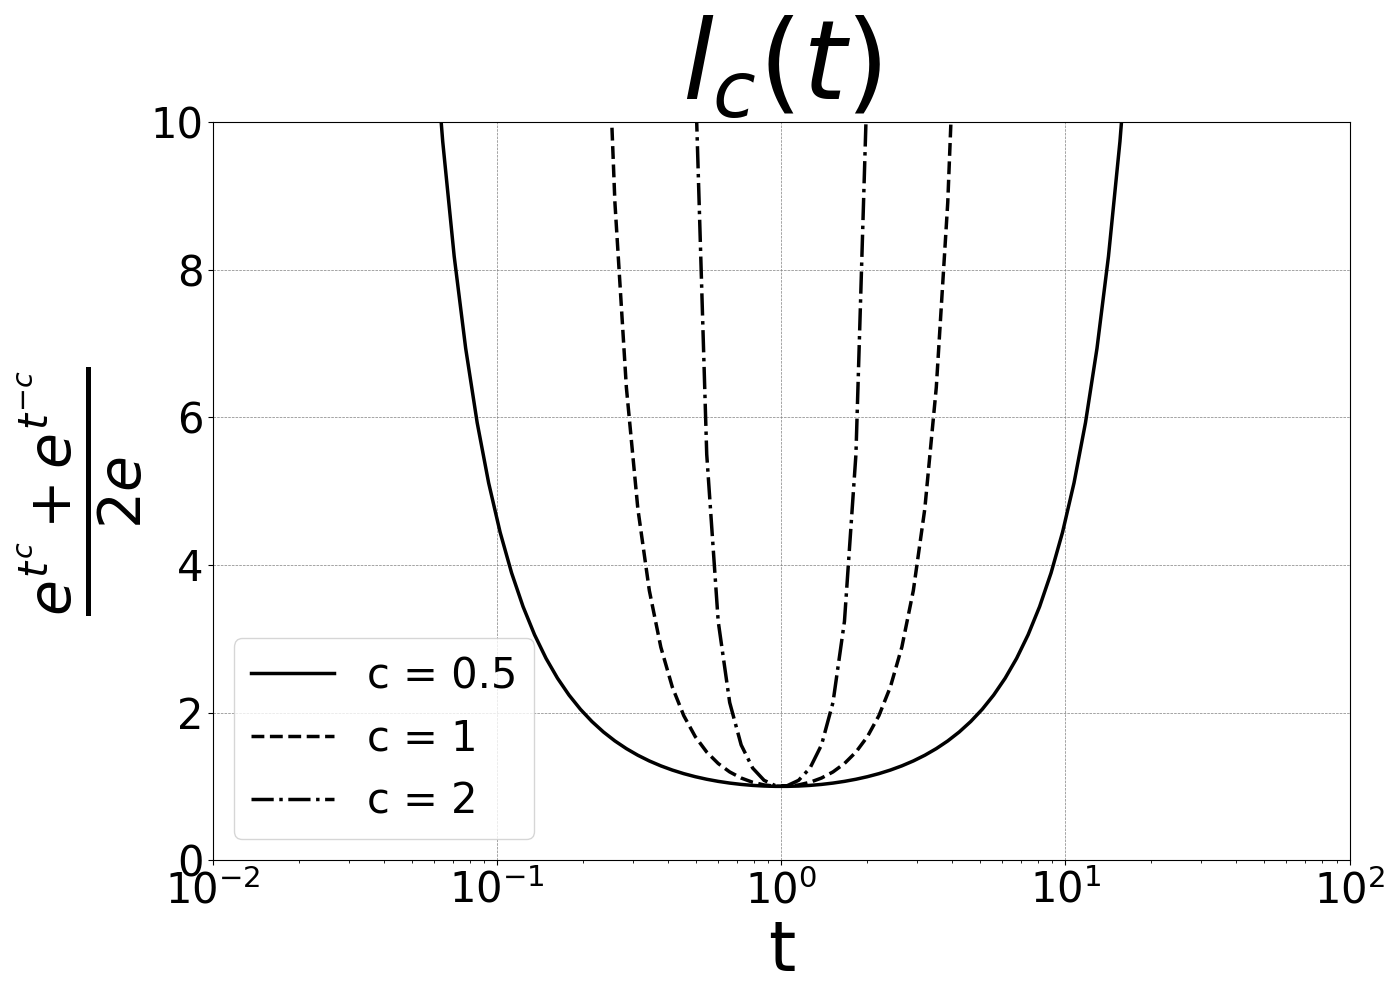
\includegraphics[width = .32\textwidth]{../figures/Figure_1a_bw.png}}
\label{fig:gt_loss}
\subcaptionbox{Normalized length as a function of unnormalized length \label{elephant}}
{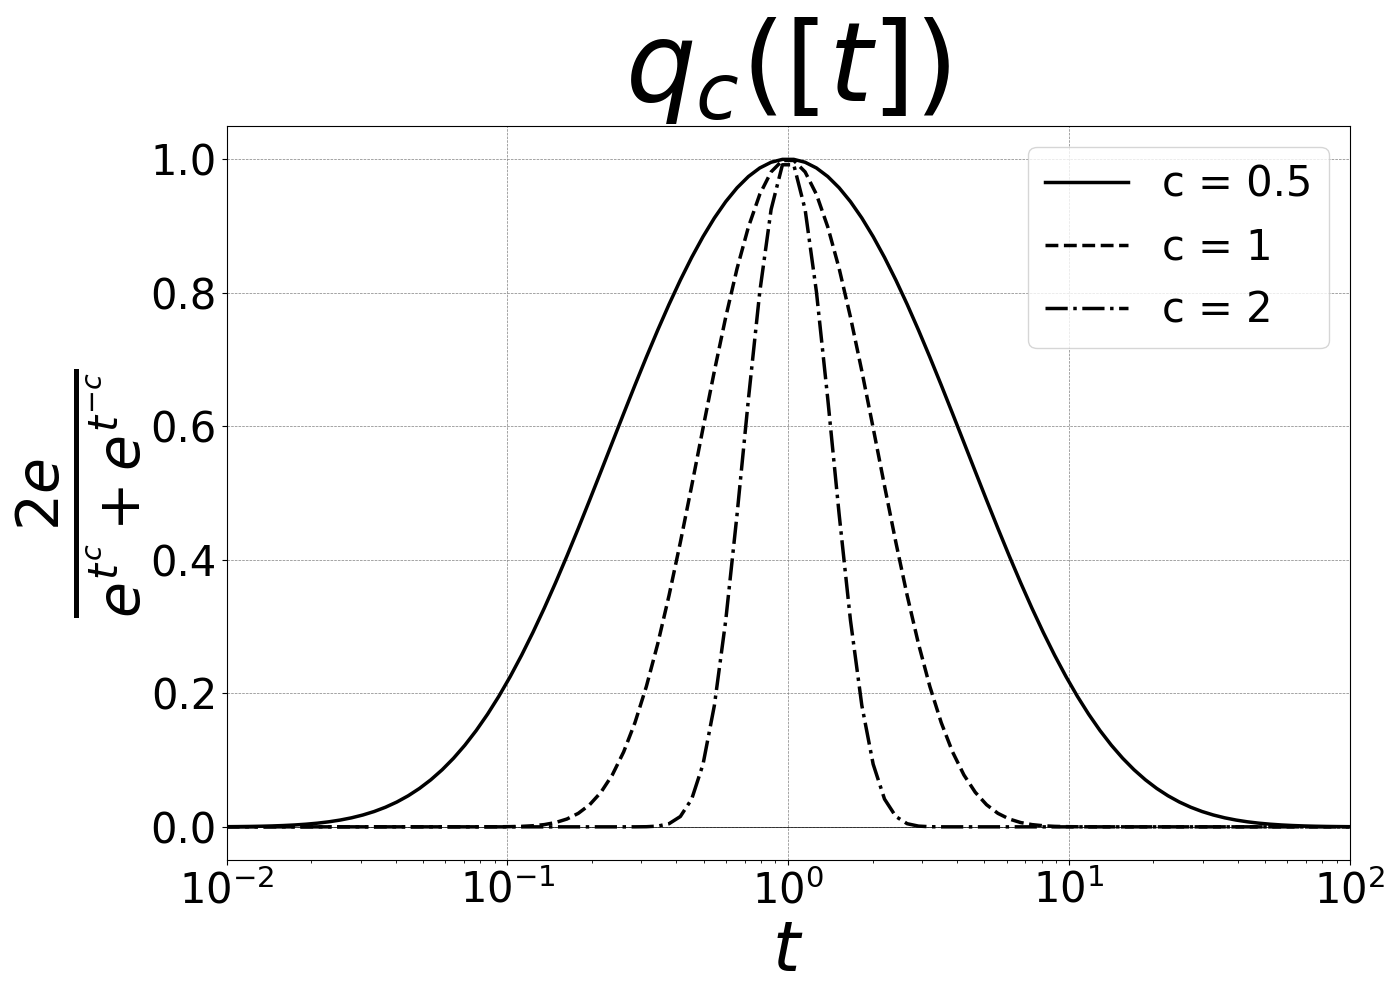
\includegraphics[width = .32\textwidth]{../figures/Figure_1b_bw.png}}
\subcaptionbox{Basis pursuit loss \label{snootfellow}}
{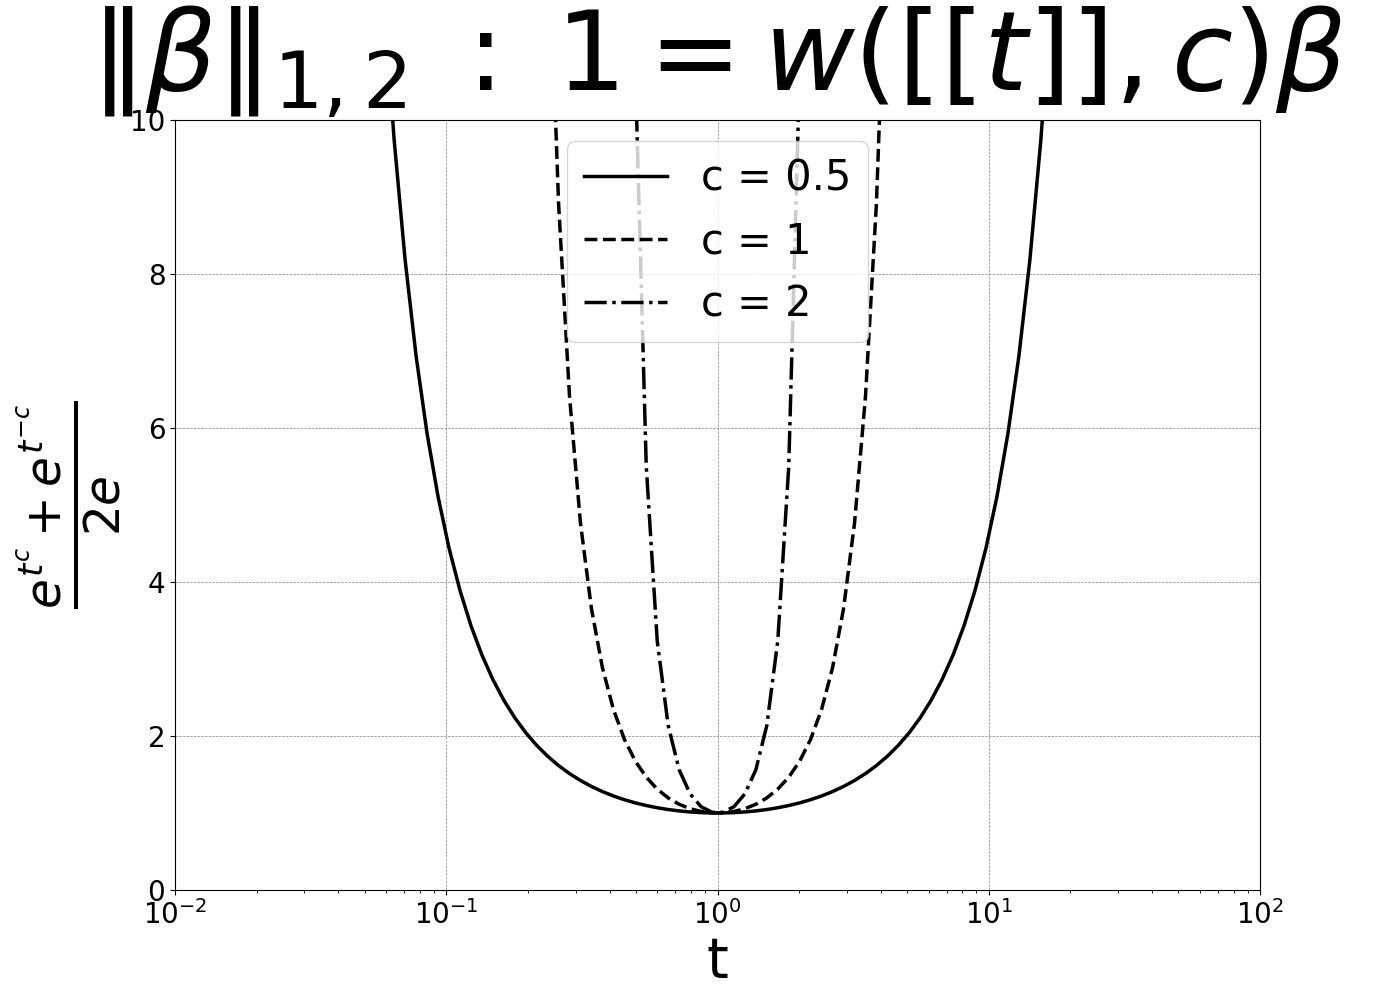
\includegraphics[width = .32\textwidth]{../figures/Figure_1c_bw.png}}
\caption{Plots of ground truth loss, normalized length, and basis pursuit loss for different values of $c$ in the one-dimensional case $D = 1$.
The two losses are equivalent in the one-dimensional case.}
\label{fig:losses}
\end{figure}

\subsection{Isometry pursuit}

Isometry pursuit is the application of multitask basis pursuit to the normalized design matrix $w(X, c)$ to identify submatrices of $ X$ that are as orthonormal as possible.
Define the multitask basis pursuit penalty 
\begin{align}
\label{eq:bp}
\| \cdot \|_{1,2}: \mathbb R^{P \times D} &\to \mathbb R^+ \\ 
\beta &\mapsto  \sum_{p=1}^P  \|\beta_{p.}\|_2.
\end{align}
Given a matrix $Y \in \mathbb R^{D \times D}$, the multitask basis pursuit solution is
\begin{align}
\label{prog:multitask_basis_pursuit}
\widehat \beta_{MBP} (X, Y)  := \arg \min_{\beta \in \mathbb R^{P \times D}} \| \beta \|_{1,2} \; : \;Y =  X \beta.
\end{align}
Isometry pursuit is then given by
\begin{align}
\label{prog:isometry_pursuit}
\widehat \beta_c ( X) := \widehat \beta_{MBP} ( w(X,c), I_D )
\end{align}
where $I_D$ is the $D$ dimensional identity matrix and recovered functions are the indices of the dictionary elements with non-zero coefficients.
That is, they are given by $S(\beta)$ where
\begin{align}
S: \mathbb{R}^{P \times D} &\to \binom{[P]}{D} \\
\beta &\mapsto \left\{ p \in [P] :  \|\beta_{p.}\| > 0 \right\}.
\end{align}
\begin{algorithm}[H]
\caption{\isometrypursuit(Matrix ${X} \in \mathbb{R}^{D \times P}$, scaling constant $c$)}
\begin{algorithmic}[1]
\STATE {Normalize} $X_c = w({X},c)$
\STATE {Optimize} $\widehat \beta = \widehat \beta_{MBP} (X_c, I_D)$
\STATE {\bf Output} $\widehat{S} = S (\widehat \beta)$
\end{algorithmic}
\end{algorithm}

\subsection{Theory}

The intuition behind our application of multitask basis pursuit is that submatrices consisting of vectors which are closer to 1 in length and more orthogonal will have smaller loss.
A key initial theoretical assertion is that \isometrypursuit~ is invariant to choice of basis for $ X$.
\begin{proposition}
\label{prop:basis_pursuit_selection_invariance}
Let $U \in \mathbb R^{D \times D}$ be orthonormal.
Then $S(\widehat \beta  (U  X)) = S(\widehat \beta ( X))$.
\end{proposition}
A proof is given in Section \ref{proof:basis_pursuit_program_invariance}.
This has as an immediate corollary that we may replace $I_D$ in the constraint by any orthonormal $D \times D$ matrix.

When a rank $D$ orthonormal column-submatrix $X_{S}$ exists, a minimizer of Program \ref{prog:multitask_basis_pursuit} consists of the inverse of this submatrix.
\begin{proposition}
Let $w_c$ be a normalization satisfying the conditions in Definition \ref{def:symmetric_normalization}.
Let $X \in \mathbb R^{D \times P}$ contain an orthonormal $D \times D$ matrix $X_S$.
Then $S \in \mathcal S_{IP} (X)$.
\label{prop:unitary_selection}
\end{proposition}
However, this solution is not necessarily unique.
\begin{proposition}
\end{proposition}
Proofs of these propositions are given in Section \ref{sec:local_isometry_proof}, with corresponding experimental results in Section \ref{sec:experiments}.

Non-unique solutions to \ref{prog:isometry_pursuit} are subtly more common than in standard lasso theory.
Recall that, given a design matrix $X$, there exists a response variable $y$ such that the lasso admits a non-unique solution if and only if the rowspan of the design matrix $X$ contains a sufficient codimension edge of the $p$ dimensional hypercube \citep{JMLR:v23:21-0420}.
This condition generalizes the previously introduced general position condition - that affinely independent columns of the design matrix guarantee non-uniqueness.
However, for Isometry Pursuit, non-unique solutions may occur even when this condition is satisfied.
A simple example -
$X =
\begin{bmatrix}
1 & 0 & \frac{\sqrt{2}}{2} & \frac{\sqrt{2}}{2}  \\
0 & 1 & \frac{\sqrt{2}}{2} & \frac{\sqrt{-2}}{2}  
\end{bmatrix}$
- can be understood as resulting from the rotation invariance Proposition \ref{prop:unitary_selection}, but more surprising examples exist.
 
%While this Proposition falls short of showing that an orthonormal submatrix will be selected should one be present, it provides intuition justifying the preferential efficacy of \isometrypursuit~ on real data.



%The requirement for existence of a response variable $y$ leading to nonunique beta is that the rowspan of the $X$ intersects the $P-1$ dimensional unit hypercube in $P$ dimensions at a point with codimension larger than the dimension of the design matrix itself.
%Here, codimension is defined as the codimension of a surface, not the linear algebra codimension.
%That is, the rowspan of $X$ must not intersect too many corners of the $P$ dimensional cube.
%For our setting, we can rewrite the multitask basis pursuit objective as $y  = \vec(I_D) \in \mathbb R^{PD}$
%\begin{align}
%y =
%    \begin{bmatrix}
%        X & 0 & 0 & \cdots & 0 \\
%        0 & X & 0 & \cdots & 0 \\
%        0 & 0 & X & \cdots & 0 \\
%      \vdots & \vdots & \vdots & \ddots & \vdots \\
%       0 & 0 & 0 & \cdots & X
%   \end{bmatrix}
%   \beta
%\end{align}
%with grouping across replicates of $X$.
%If $row(X)$ intersects the 1-ball in a location with codimension $C$, then the repeated $X$ intersects this higher-dimensional 2-1 ball in a location with codimension $D * (C -1 ) + 1$ since $C - 1$ is the rank-deficiency induced by the structure of the matrix $X$ rather than intrinsic to the $D-1$ dimensional ball.


% I dont think this is true %A grreater number of tasks increases the codimension of the combined matrix and can thus enable non-unique solutions for design matrices that would satisfy uniqueness for basis pursuit.
% Note that that given the presence of an isometry solution, for which by the rotation invariance Proposition \ref{prop:basis_pursuit_selection_invariance}, $C$ is at least $D$.

%A well-known result in Lasso literature states that if the columns of $X$ are in so-called general position (meaning that no more than $k+1$ columns are contained within any $k$ dimensional subspace, with $k < D$), then the standard lasso solution is unique.

\subsection{Optimization}

When the solution is non-unique, we naturally wonder what are the properties of the solution that we end up with, and if that solution has some stable characterization or is random across replicates.
The typical response to considerations of non-uniqueness in such problems is the characterization of the "min-norm" solution.
Group lasso's uniqueness has been studied in \citet{Mishkin2022-yf} and lasso's uniqueness has been studied in \citet{Tibshirani2012-vw}.
While in \citet{Tibshirani2012-vw} the selection of the minimum l2-norm solution (the "min-norm") solution among the lasso solution was proven for the Least Angle Regression Selection (LARS) algorithm for solving the lasso, \citet{Mishkin2022-yf} assumes that the group lasso solution is in fact min-norm prior to subsequent theoretical analyses.

Behavior of estimating algorithms in the of particular interest given the presence of non-unique solutions.
The computational estimation of the isometry pursuit solution is of particular interest because of the increased potential for non-unique solutions that comes with the increased number of tasks.



\subsection{Two-stage isometry pursuit}

Since we cannot ensure either that $|\widehat {  S}| = D$ or that a orthonormal submatrix $X_{.S}$ exists, we first use the convex problem to prune and then apply brute search upon the substantially reduced feature set.

\begin{algorithm}[H]
\caption{\tsip(Matrix ${X} \in \mathbb{R}^{D \times P}$, scaling constant $c$)}
\begin{algorithmic}[1]
\STATE $\widehat{S}_{IP} = \text{\isometrypursuit}( X, c)$
\STATE $\widehat{S} = \text {\brute}({X}_{.\widehat{S}_{IP}}, l_c)$
\STATE {\bf Output} $\widehat{S}$
\end{algorithmic}
\end{algorithm}

Similar two-stage approaches are standard in the Lasso literature \cite{Hesterberg2008-iy}.
This method forms our practical isometry estimator, and is discussed further in Sections \ref{sec:discussion} and \ref{sec:deep_dive}.